% Metódy inžinierskej práce

\documentclass[10pt,twoside,slovak,a4paper]{article}

\usepackage[slovak]{babel}
%\usepackage[T1]{fontenc}
\usepackage[IL2]{fontenc} % lepšia sadzba písmena Ľ než v T1
\usepackage[utf8]{inputenc}
\usepackage{graphicx}
\usepackage{url} % príkaz \url na formátovanie URL
\usepackage{hyperref} % odkazy v texte budú aktívne (pri niektorých triedach dokumentov spôsobuje posun textu)

\usepackage{cite}
%\usepackage{times}



\title{Herné umenie\thanks{Semestrálny projekt v predmete Metódy inžinierskej práce, ak. rok 2022/23, vedenie: Meno Priezvisko}} % meno a priezvisko vyučujúceho na cvičeniach

\author{Marek Fiľo\\[2pt]
	{\small Slovenská technická univerzita v Bratislave}\\
	{\small Fakulta informatiky a informačných technológií}\\
	{\small \texttt{xfilo@stuba.sk}}
	}

\date{\small 30. september 2022} % upravte



\begin{document}

\maketitle

\begin{abstract}


Cieľom tohto článku je priblížiť čitateľovi pojemy \emph{Herné umenie}, \emph{Herný umelec}a pribížiť časti, na ktoré sa delí. Pozrieme sa aj na to ako herné umenie ovplyvňuje popularitu hry a či je to hlavný faktor, ktorý ovplyvňuje úspešnosť hry.
\end{abstract}




\section{Úvod} \label{začiatok}
Vznik herného umenia ako ho poznáme dnes podmienil vznik počítačov a ich rozšírenie medzi širokú verejnosť.
Pod slovným spojením  \emph{Herné umenie} si môže niekto predstaviť perfektne zahranú hru či už šachu alebo niektorej z moderných počítačových hier. My pod týmto názvom rozumieme vizuálne prevedenie hry. Všetko čo vidíme na obrazovke alebo aj na našom stole je výsledkom práce herných umelcov, ktorých úlohou bolo vytvoriť návrhy a výsledné prevedenia toho čo vidíme, tak aby to odpovadalo téme hry, časovému obdobiu v ktorom sa hra odohráva a taktiež žánru hry.














\section{Herný umelec} \label{pokračovanie}
Herný umelec je človek, ktorý ma na svedomí vzhľad prostredia, postáv a všetkých ostatných prvkov, ktoré sa v hre vyskytujú. Umelcov rozdeľujeme na nasledovné kategórie.
\paragraph{Koncepčný umelec} Dáva základnú podobu všetkému čo sa v hre vyskytuje. S jeho návrhmi pracujú ostatný umelci a dávajú im finálnu podobu.
\cite{kon}

\paragraph{Umelec prostredia} Vytvára prostredie, modeluje 3D modely prvkov, ktoré sa v ňom nachádzajú napr. strom, dom. Všetko čo vidíme na pozadí aj miesta, po ktorých sa pohybujeme sú výsledkom práce tohto človeka.
\cite{spectrum}

\paragraph{Charakterový umelec} Výtvára vzhľad postáv. Pretvára ilustrácie alebo skenuje reálnych ľudí, ktorý sa v hre objavujú.
\cite{spectrum1}

\paragraph{Animátor postáv} Špeciálny typ 3D animátora, ktorý vdychuje život postavám. 
\cite{spectrum2}

\paragraph{FX animátor}Je zodpovedný za všetky špeciálne efekty ako napríklad výbuchy, oheň a mnohé iné. Jeho úlohou je aby tieto efekty vyzerali reálne a divák si nemyslel že sú počítačivo generované.
\cite{spectrum3}

\section{Ako sa stať herným umelcom}
Herné umenie ako každé iné si vyžaduje kreativitu a kúsok talentu. Najprv sa treba zamerať na základy ako sú kreslenie, perspektíva, tieňovanie a hĺbka. Neodmysliteľnou súčasťou je práve kreslenie, treba sa v ňom zlepšovať a cvičiť najlepšie každý deň. Ďalším krokom je práca s programami na tvorbu grafiky, prit výbere programu, v ktorom budete pracovať záleží na tom či chcete tvoriť 2D alebo 3D grafiku. Jeden z najznámejších porgramov pre 2D grafiku je Adobe Photoshop, pre 3D grafiku to je Maya a 3DS Max, ktoré sú používané mnohými spoločnosťami.
\cite{1}






\section{2D štýly herného umenia}
\cite{2D}
\paragraph{Pixel art}
Jeden z najpopulárnejších štýlov 2D. Mnoho ľudí si Pixel art spája s prvými videohrami ale tento šlýl má slušné zastúpenie aj v tejto dobe. Takáto hra v ľuďoch vzbudzuje nostalgiu hlavne spojenú s hrou Pokemon.


\paragraph{Vector art}
Hry vytvorené týmto štýlom sú na trhu veľmi dlho aj keď nie sú tak populárne ako hry s pixel grafikou. Je to najmä preto lebo neexistuje veľa programov a metód na prácu s vektormi. Obrázky sa nerozdeľujú na jednotlivé pixely ale ukladajú sa pomocou geometrických tvarov. Výhodou je menšia veľkosť obrázkov avšak takýchto hier je v súčastnosti málo.

\paragraph{Cutout art}
Ako už meno napovedá, tento štýl napodobňuje obrázky nakreslené na papieri a vložené do hry. Obraz výrezu ostáva nemenný, mení sa jeho poloha aby sa simulovala akcia alebo obraz výrezu môže byť nahradený iným výrezon na simuláciu zmeny stavu. Výsledkom je hra s naozaj jedinečným vzhľadom.


\paragraph{Cel Shading art}
Tento štýl sa snaží vytvoriť 3D modely a objekty tak, aby vyzerali ako 2D.


\paragraph{Monochromatic art}
Vyznačuje sa veľmi limitovanou paletou farieb, zväčša 1 alebo 2 farby. A však v hre je použitých mnoho odtieňov pre lepšie rozlišovanie medzi objektami. Tieto hry často pôsobia tajomne alebo desivo a z vlastnej skúsenosti viem povedať že v hráčovi vzbudzujú nezabudnuteľné pocity.

\paragraph{Flat art}
Postavy v hre sú bez hĺbky a objemu. Nenájdeme tu žiadne reálne prvky a ani prvky fyziky. V tomto štýle majú umelci takmer úplnú voľnosť.

\paragraph{Doodle art}
Tento štýl je definovaný hlavne svojím osobitým vzhľadom. Postavy a prvky prostredia majú netradičný vzhľad a často sú zložené z viacerých samostatných prvkov.
Doodle jump


\section{3D štýly herného umenia}

\paragraph{Realizmus}
Zámerom je vytvoriť grafiku, ktorá vyzerá čo najvia podobá na realitu. Najväčšie AAA tituly vychádzajú v tomto štýle. Časová línia môže byť zasadená do ktorého koľvek obdobia, dej a žáner hry sa s realitou nemusia vôbec podobať. 


\paragraph{Fantasy realizmus}
Tento štýl sa od predchádzajúceho odlišuje najmä v žánre hier, v ktorých sa vyskytuje. Grafika sa podobá realite ale príbeh a dej nemá s realitou nič spoločné. Hráčovi vie priniesť maximálny herný zážitok spolu s umelckou hodnotou.


\paragraph{Low Poly}
Podstatou tohto štýlu je zobrazovanie objektov pomocou mnohouholníkov. Každý má jednu farbu, ktorá sa nemení. Z názvu by sa dalo usúdiť že sa jedná o štýl s malou kvalitou obrazu ale nie je to tak, v jednej hre sa môže vyskytovať okolo milióna jednotlivých tvarov.


\paragraph{Hand-Painted}
Základom je textúra maľovaná voľnou rukou bez zásahu geometrie. Najčastejšie sa používa pri fantasy a strategických hrách. Často sa takéto hry graficky podobajú na komiks, rozprávku alebo dokonca aj realitu.

\paragraph{Cartoon}
Dalo by sa povedať že tento štýl zahŕňa Low Poly aj Hand-Painted. Niekedy sú textúry pre takúto hru ručne maľované ale nemusí to tak byť. Hry sú farebnejšíe a taktiež o niečo málo grasficky jednoduchšie. Vývoj nie je tak dlhý práve vďaka jednoduchosti detailov, narozdiel od hier s realistickou grafikou kde sa musí dbať na každý detail.



\section{Prečo sa populárne hry stali populárnymi}
Na začiatok treba povedať že väčšia časť tohto textu sú moje názory a to ako vidím danú hru ja. V tabuľke sú hry, ktoré som vybral na porovnávanie a rozoberanie štýlu. Údaje sú z platformi Steam zo dňa 27.11., všetky sa nachádzali v top 100 najhranejších hier za daný deň.

\begin{center}
\begin{tabular}{ |c| c| }
\hline
 Hra & Denne maximum 27.11. \\
\hline
 CS:GO & 1053250 \\
\hline
 COD:Modern Warfare II & 373000 \\
\hline
 GTA 5 & 162000 \\
\hline
 Rust & 110000 \\
\hline
 Civilization VI & 90000 \\
\hline
 WarThunder & 66500 \\
\hline
 Euro Truck Simulator 2 & 43000 \\
\hline
 Zaklínač 3:Divoký hon & 33000 \\
\hline
 Phasmophobia & 20000 \\
\hline
 God of War & 18000 \\
\hline
\end{tabular}
\end{center}

\paragraph{CS:GO}
Novšia verzia klasiky, ktorú hral asi každý. Patrí k najhranejším hrám na svete a otázka je, či je to kvôli dizajnu a grafike. V rámci štýlov by som túto hru zaradil do 3D realizmu. Umelecké spracovanie nie je ničím špeciálne a textúry sú zväčša jednoduché a prisbôsobené hlavnému cieľu hry a to je súťaživosť. Nepotrebuje špeciálne efekty blata alebo snehu, postačuje úprava fyziky keď sa hráč nachádza v zložitejšom teréne. Hra ponúka nekonečnú zábavu, ak sa to vôbec dá nazvať zábavou, tradíciu, rôzne vzhľady zbraní a postáv, možnosť zlepšovania sa a hru viacerých hráčov a to je podľa mňa to, prečo je CS:GO populárne aj po mnohých rokoch na trhu.

\paragraph{COD:Modern Warfare II}

\paragraph{GTA 5}

\paragraph{Rust}

\paragraph{Civilization VI}
Túto hru by som zaradil k 3D cartoon hrám. Grafické spracovanie je príjemné na pohľad a novému hráčovi umožní sa viac sústrediť na ostatné časti hry, ktoré si vyžadujú viac času na porozumenie. Modely postáv su niekdy komické ale zároveň zodpovedajú historickým osobnostiam. Ak ju porovnáme s hrou rovnakého žánru Hearts of Iron, ktorá je spracovaná realisticky, tak by som povedal že Civilization je prehľadnejšia a z hľadiska umenia aj zaujímavejšia. Hra ponúka všetko čo každá strategická hra a navyše pridáva neobyčajné spracovanie, čiže by sa dalo povedať že je populárna vďaka svojmu hernému umeniu

\paragraph{WarThunder}

\paragraph{Euro Truck Simulator 2}

\paragraph{Zaklínač 3:Divoký hon}

\paragraph{Phasmophobia}

\paragraph{God of War}





















%\acknowledgement{Ak niekomu chcete poďakovať\ldots}


% týmto sa generuje zoznam literatúry z obsahu súboru literatura.bib podľa toho, na čo sa v článku odkazujete
\bibliography{literatura}
\bibliographystyle{abbrv} % pabbrvrípadne alpha, abbrv alebo hociktorý iný
\begin{figure}[!ht]
\begin{center}
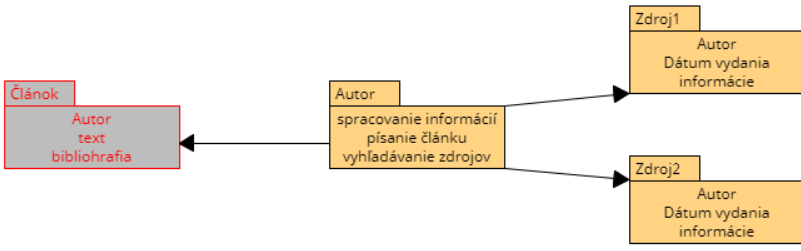
\includegraphics[width=12cm]{diagram novy.png}
\caption{Diagram}
\end{center}
\end{figure}

\end{document}
